\documentclass[12pt]{article}
\usepackage[left=1.0in, right=1.1in, top=1in, bottom=1in, noheadfoot]{geometry}
\usepackage[table]{xcolor}
\usepackage[utf8]{inputenc}
\usepackage{amssymb,amsfonts,graphicx}
\usepackage{hyperref}
\usepackage{tikz}
\usetikzlibrary{shapes.geometric, arrows}
%\setlength{\tabcolsep}{1pt}
%\usepackage{subcaption}
%\usepackage{tabu}
%\graphicspath{{./}{./figures/}{../figures/}}
\DeclareGraphicsExtensions{.pdf,.png,.jpg}
\usepackage{graphicx}
\usepackage{graphics}
\usepackage{longtable}
%\usepackage{natbib}
\usepackage{amsmath}
\usepackage{multirow}
%\usepackage[square,sort,comma, numbers]{natbib}
\setlength{\arrayrulewidth}{0.1mm}
\setlength{\tabcolsep}{6pt}
\renewcommand{\arraystretch}{1.3}
\graphicspath{{images/}}
%\title{
%	{\LARGE \textbf{Thermodynamic assessment of the Ni-Zr system}}\\
%% Warning: check the title --if Ni-Zr or Al-Ni-Zr
%%	{\large Indian Institute of Technology Madras}\\
%}
%
%\author {Asmita Jana}
%\date {23rd September 2016}
\begin{document}
%\maketitle
\begin{titlepage}
    \begin{center}
        \vspace*{5cm}
        
        {\LARGE \textbf{Precipitation sequence in Niobium-alloyed \\
	ferritic stainless steel}}
        
	\vspace{1.0cm}
	\textit{a report by}
        
        \vspace{1.5cm}
        
        \textbf{ASMITA JANA} \\
	\textbf{ (MM12B006)}\\
        
        \vspace{3.0cm}
        \textit{Based on the work by}\\

        
        \vspace{1.5cm}
        
        \textbf{Fujita et.al.*}\\
	 
	\vspace{5cm}

	\footnotesize{*Fujita, Nobuhiro, H. K. D. H. Bhadeshia, and Masao Kikuchi. "Precipitation sequence in niobium-alloyed ferritic stainless steel." Modelling and Simulation in Materials Science and Engineering 12.2 (2004): 273.}
    \end{center}
\end{titlepage}
%\begin{document}
\newpage

%-------------------------------------------------------------------
\section{Introduction}

   As the world becomes more sustainable in terms of energy usage, every industry is on the lookout for energy conserving processes and products. In the automobile industry, a higher temperature of exhaust gas implies better fuel efficiency. The next step, then becomes a search of materials with better high temperature strength and resistance to thermal fatigue. Niobium as a solute in ferritic stainless steel gives these required properties and is used extensively.

 However, it has been noted that Niobium forms varieties of precipitates when exposed to high temperatures for a longer period of time. The precipitates formation can critically affect the performance of these materials. Hence it has become crucial to study the precipitation kinetics of the intermetallics. One such study by Fujita \textit{et. al.} has been done and is analysed in this report.


\section{Experiments done}

 An alloy with a nominal composition of 19Cr-0.8Nb wt.\% is taken. Vacuum melting was done followed by heating at 1250$^\circ$C for 30 minutes in an Ar atmosphere. It was then hot-rolled and normalized to 900$^\circ$C. Annealing was done at 1000$^\circ$C for 10 minutes and subsequently water quenched. Machining was done and the samples were then subjected to isothermal heat treatments at temperatures of 950$^\circ$C and 1000$^\circ$C for 500 hours. 

X-ray diffraction studies were done and precipitates formed were noted. Transmission electron microscopy, electron diffration and energy dispersive studies were used with carbon extraction replicas to characterize the microstructures and particle sizes.

\section{Experimental results}

 The chemical compostition obtained using XRD has been listed in Table \ref{tab:nom}. XRD studies and chemical analyses of the residues from the samples have characterised the precipitates forming at different conditions. They have been listed in \ref{tab:prec}.
%--------------------------------------------------------
\begin{table}
\centering
%\hspace*{-3em}
\caption{Chemical composition (wt.\%) of the ferritic stainless steel}
%\hspace*{-5em}
\begin{tabular}{ l l l l l l l }
\hline
\hline
Nominal & C & Si & Mn & Cr & Nb & N \\
\hline
19Cr-0.8Nb & 0.014 & 0.2 & 0.3 & 19.6 & 0.78 & 0.016 \\
\hline
\hline
\end{tabular}
\label{tab:nom}
\end{table}
%----------------------------------------------

%--------------------------------------------------------
\begin{table}
\centering
\hspace*{-5em}
\caption{Presence of precipitates in samples at different experimental conditions: VW, W,S,VS stand for very weak, weak, strong and very strong X-ray intensities}
\hspace*{-5em}
\begin{tabular}{ c c c c c }
\hline
\multicolumn{2}{c}{Aging conditions} &  \multicolumn{3}{c}{Precipitates detected}\\
Temperature ($^\circ$C) & Time (h) & Nb(C,N) & Fe$_3$Nb$_3$C & Fe$_2$Nb \\ \hline
As annealed &  & S & VS & W \\
at 1000$^\circ$C & & & & \\ 
 & 1 & VS & VS & VS \\
 & 8 & S & VS & W \\
950 & 20 & S & VS & W \\
 & 50 & S & VS & VW \\
 & 100 & VW & VS & - \\
1000 & 20 & W & VS & - \\ \hline
\end{tabular}
\label{tab:prec}
\end{table}
%----------------------------------------------
It is concluded that M$_6$C might be an equilibrium phase given that it was observed only at the coarsening stage. Radii of the precipitates were calculated by measuring the area in the 2D image and equating it to that of a circle with equivalent area.

 At the initial stages, intensities from Nb(C,N), Fe$_2$Nb and Fe$_3$Nb$_3$C were found to be strong. As time increased in the aging process, intensities of the Nb(C,N) and Fe$_2$Nb decreased with increase for Fe$_3$Nb$_3$C. In the extracted residues, it was found that most of Nitrogen had precipitated as NbN, implying that NbC dissolves while NbN remains. The extracted residue showed equivalent atomic fractions of Fe and Nb implying that Fe$_3$Nb$_3$C is one of the final phases remaining. The precipitation sequence obtained is as follows:
\newline
$\alpha \rightarrow \alpha$ + Nb(C,N) + Fe$_2$Nb + Fe$_3$Nb$_3$C $\rightarrow \alpha$ +NbN + Fe$_3$Nb$_3$C.


Under the TEM, the precipitates were found to be more spherical than needle like even in case of aging for 20 hours at 950$^\circ$C.

\section{Model used}
\subsection{Nucleation}
In order to obtain the nucleation rates $I$ for each precipitate, the classical nucleation theory was used. The nucleation rate is given by Equation \ref{eq:nucl}.

\begin{equation}
I=\bigg(1-\frac{V^\beta}{V^{\alpha \beta}}\bigg)N_0\frac{kT}{h}exp\bigg(-\frac{G^*+Q^*}{RT}\bigg)
\label{eq:nucl}
\end{equation}
where $G^*$ is given by \ref{eq:g}
\begin{equation}
G^*=\frac{16\pi \sigma^3}{3\Delta G_V^2}
\label{eq:g}
\end{equation}
Here, $V^\beta$ and $V^{\alpha \beta}$ are instantaneous and equilibrium volume fractions of the precipitate. $N_0$ and $Q^*$ are the number density of nucleating sites and activation energy respectively. $\sigma$ and $\Delta G_V$ are interfacial energy and volume Gibbs energy change. 

\subsection{Growth}

For growth by diffusion, the concentration flux directly feeds the precipitate growth. This can be shown in Figure \ref{fig:prec_g}. The equation governing the growth in case of binary alloys is given by Equation \ref{eq:gro}. 

%--------------------------------------
\begin{figure}
\centering
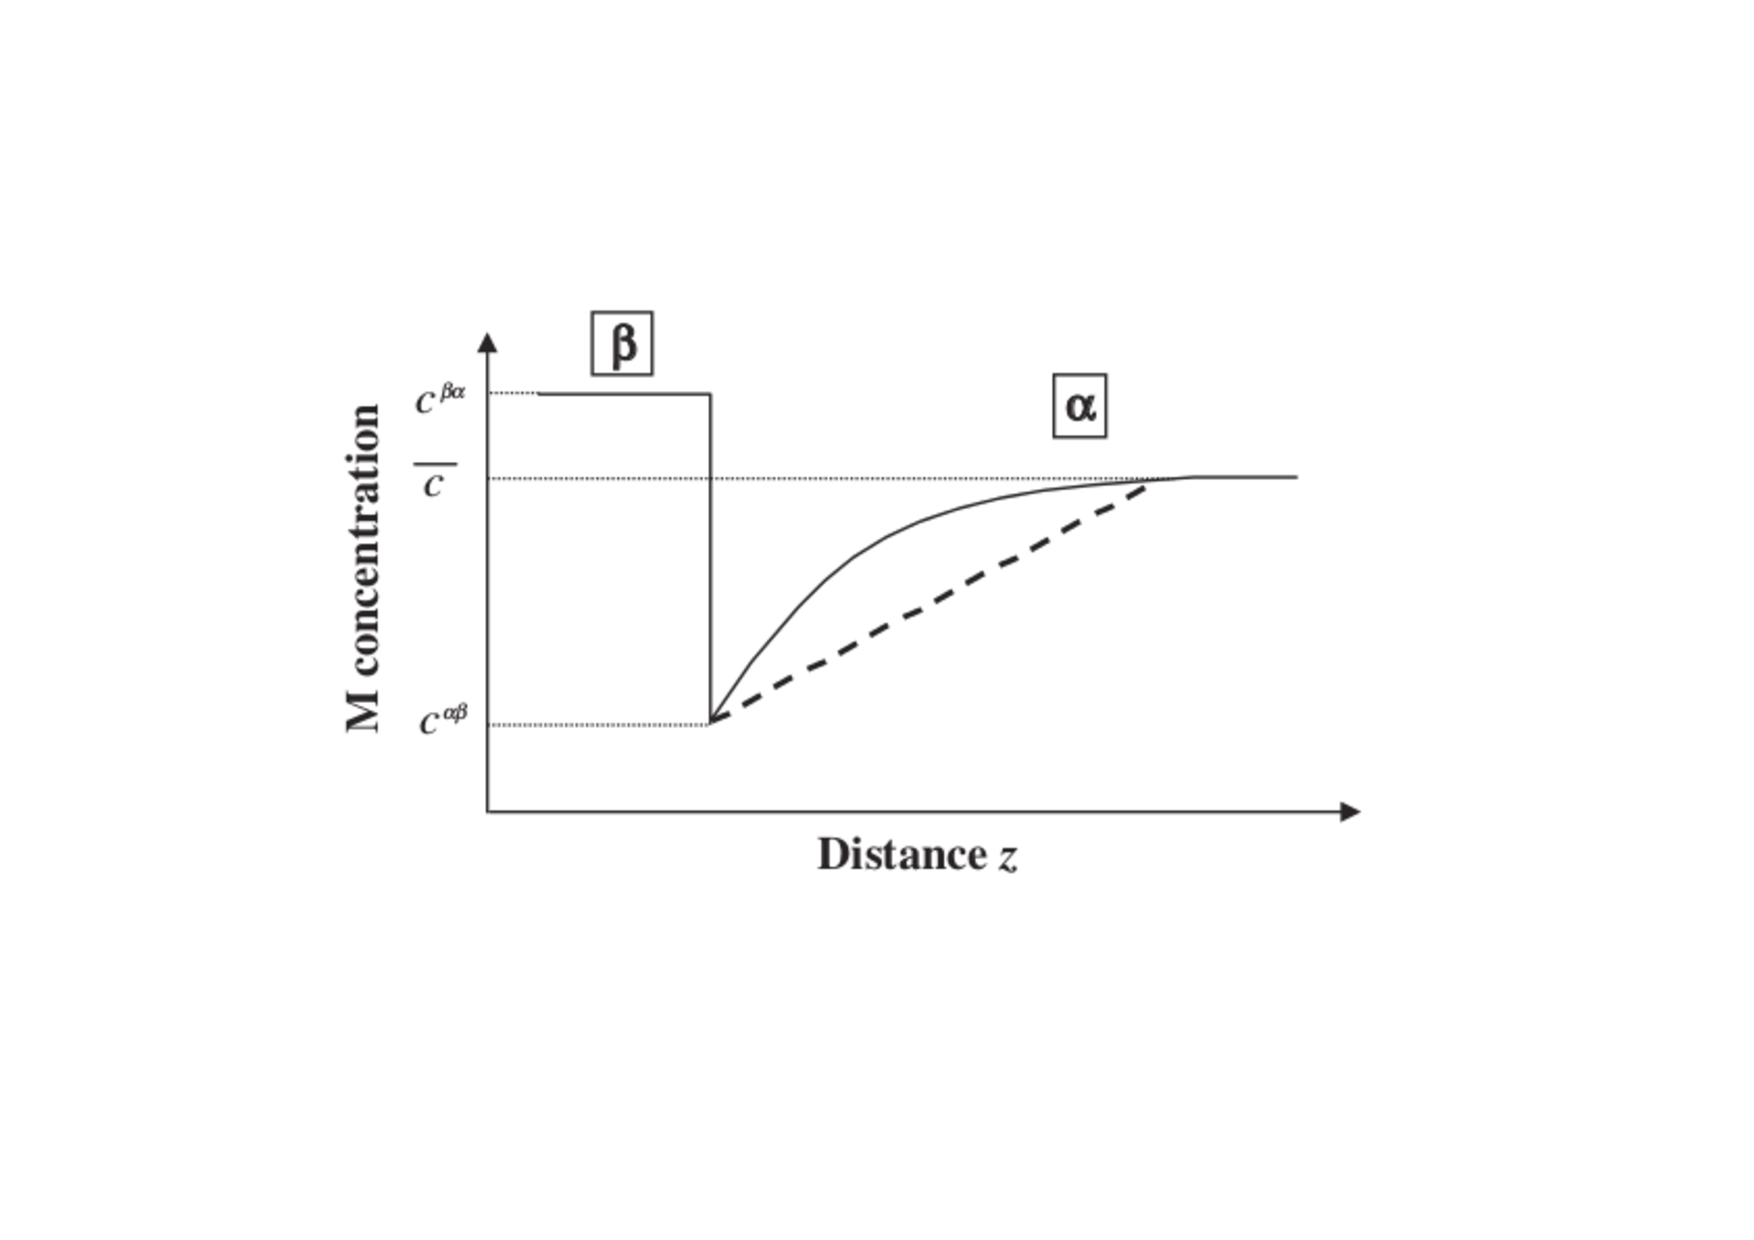
\includegraphics[width=14cm]{prec.pdf}
\caption{Schematic showing precipitate formation in a binary alloy}
\label{fig:prec_g}
\end{figure}
%---------------------------------------
\begin{equation}
v(c^{\beta \alpha}-c^{\alpha \beta})=-D\frac{\partial c}{\partial z}
\label{eq:gro}
\end{equation}
 
Here, $D$, $v$, $c^{\beta \alpha}$, $c^{\alpha \beta}$, $\frac{\partial c}{\partial z}$ are diffusion coefficient, growth velocity, concentrations at equilibrium and concentration gradient. 
For a ternary system, there will be diffusion of two components. Hence, we would need to satisfy two conservation equations. For a carbide, MC in a matrix, Equations \ref{eq:terna} and \ref{eq:ternb} will be used.

\begin{equation}
v(c_M^{\beta \alpha}-c_M^{\alpha \beta})=-D_M\nabla c_M
\label{eq:terna}
\end{equation}

\begin{equation}
v(c_C^{\beta \alpha}-c_C^{\alpha \beta})=-D_C\nabla c_C
\label{eq:ternb}
\end{equation}

Owing to Carbon being an interstitial atom, $D_C >> D_\mathrm{Nb}$. Thus for the equations to be satisfied, the C gradient should be low enough such that the flux extent of C and Nb almost match. 

The process can be clearly delinated from Figure \ref{fig:diff}. $\bar{c_C}$ and $\bar{c_M}$ represent the average composition of C and M atoms in the matrix. The intersection of the vertical line from a intersecting the phase boundary gives the initial C concentration. This method ensures the lowest possible difference in C content between the precipitate and the matrix, conserving the equations. As diffusion proceeds, tie-line moves from b to c, decreasing the flux of M atoms subsequently. Simultaneously, the average concentration of the matrix moves from a to c, due to solute depletion. The final equilibrium state thus ends up being c. 

%--------------------------------------
\begin{figure}
\centering
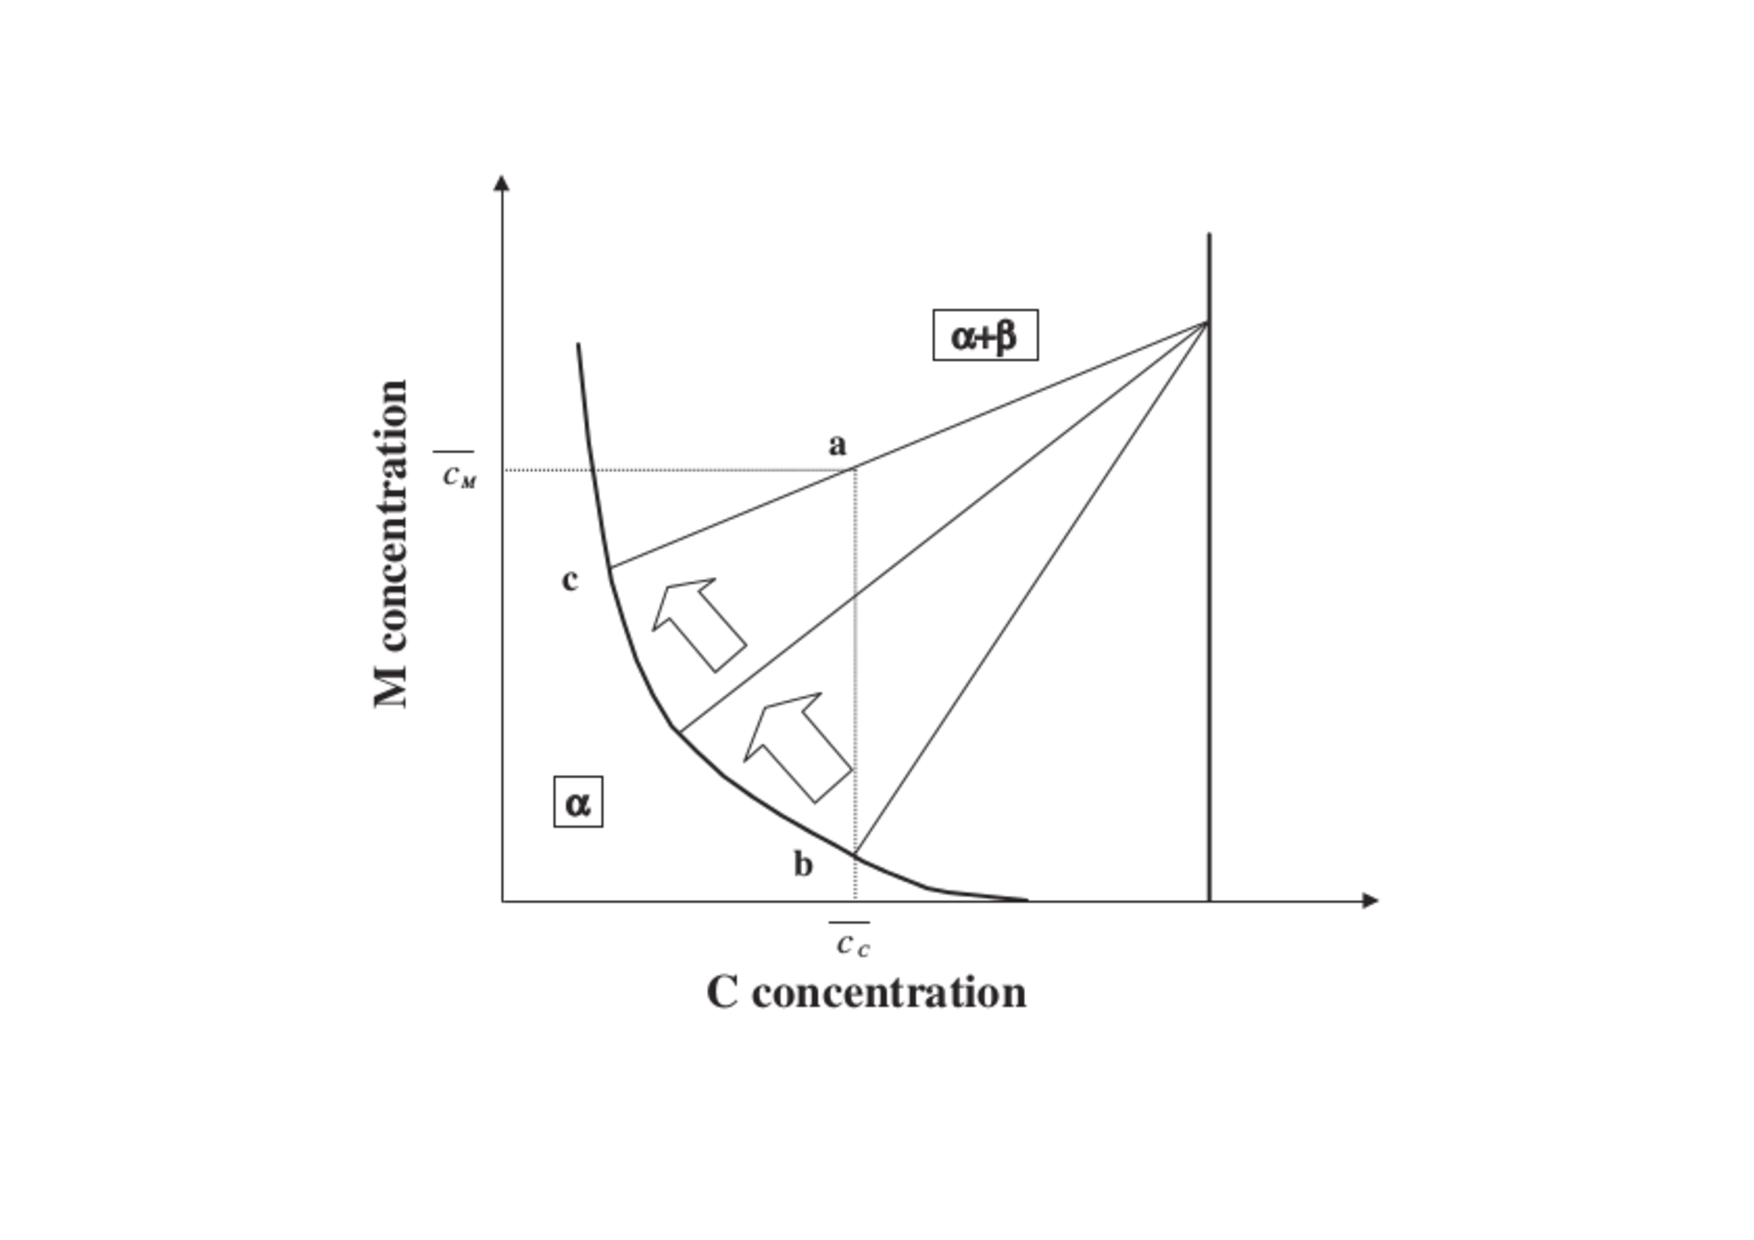
\includegraphics[width=14cm]{phd.pdf}
\caption{Diffusion conditions in a MC precipitate and matrix system}
\label{fig:diff}
\end{figure}
%---------------------------------------
 When the diffusion-controlled growth theory is applied to this situation, we end up with a solution given in Equation \ref{eq:zz}.
\begin{equation}
z=\alpha_3\sqrt{Dt}
\label{eq:zz}
\end{equation}

where $\alpha_3$ is given by
\begin{equation}
\alpha_3=\sqrt{2\frac{\bar{c}-c^{\alpha \beta}}{c^{\beta \alpha}-\bar{c}}}
\label{eq:zzz}
\end{equation}

\subsection{Capillarity}

Thermodynamics deals with systems having phases of infinite curvature. In real world, it is found that curvature effects have a significant role to play in energetics and thus consequently in thermodynamics and kinetics of processes.

The Equation \ref{eq:curv} is followed when including curvature effects.
\begin{equation}
c_{r,\mathrm{M}}^{\alpha \beta}=\bigg(1+\frac{\sigma}{kT}\frac{v^\beta}{r}\frac{1-c_{\mathrm{M}}^{\alpha \beta}}{c_{\mathrm{M}}^{\beta \alpha}-c_{\mathrm{M}}^{\alpha \beta}}\bigg)c_{\mathrm{M}}^{\alpha \beta}
\label{eq:curv}
\end{equation}

The equation is incorporated when calculating the phase boundaries giving modified ones for every radius of curvature.
The capillarity effect reduces the probability of having an excessive amount of small sized precipitates. Also the larger the precipitate, the lower is the solute content at its interface. This drives coarsening ever further.

\section{Calculations done}

To get the volume Gibbs energy, the CALPHAD description was used for Nb(C,N) and for Laves phase and M$_6$C carbide, their solubility products were used. The precipitation was assumed to take place in the Fe-Nb-C system. The parameters used in this calculation were $N_0$ and $\sigma$, the number of nucleation sites and the interfacial energy respectively. These parameters were varied to get a close agreement with experimental data.

It was observed that the interfacial energy has a 15 times stronger impact than number of nucleation sites for a given magnitude change in both.

\subsection{Volume fraction and particle sizes}

Volumes fractions of each phase was calculated and plotted in Figure \ref{fig:vol} along with experimental results. A close agreement was seen. The precipitation sequence was correctly obtained using the model verifying its accuracy.
The volume fraction was found to saturate after some time. This can be understood from the fact that the dissolution of smaller particles happen simultaneously with coarsening of the large particles. The mean radius was also found to increase and then stabilize after some time as shown in Figure \ref{fig:size}. After a longer period of time, it was found to grow further as can be concluded from coarsening. The number density also increases to a certain level before stabilizing. Unlike the mean radius, it decreases in the time ranges when the mean radius grows. This is because coarsening results in lesser number of precipitates altogether.

%--------------------------------------------------------
\begin{table}
\centering
%\hspace*{-3em}
\caption{Results from modeling}
%\hspace*{-5em}
\begin{tabular}{ l c l }
\hline
 & Number density of sites: $N_0$ (m$^{-3}$&) \\
NbN & & $2\times10^{12}$ \\
Fe$_2$Nb & & $3\times10^{11}$ \\
Fe$_3$Nb$_3$C & & $3\times10^{12}$ \\
 & Interfacial energy: $\sigma$( J m$^{-2}$) & \\
NbN & &  0.230\\
Fe$_2$Nb & & 0.280 \\
Fe$_3$Nb$_3$C & & 0.330 \\
\hline
\end{tabular}
\label{tab:res}
\end{table}
%----------------------------------------------
%--------------------------------------
\begin{figure}
\centering
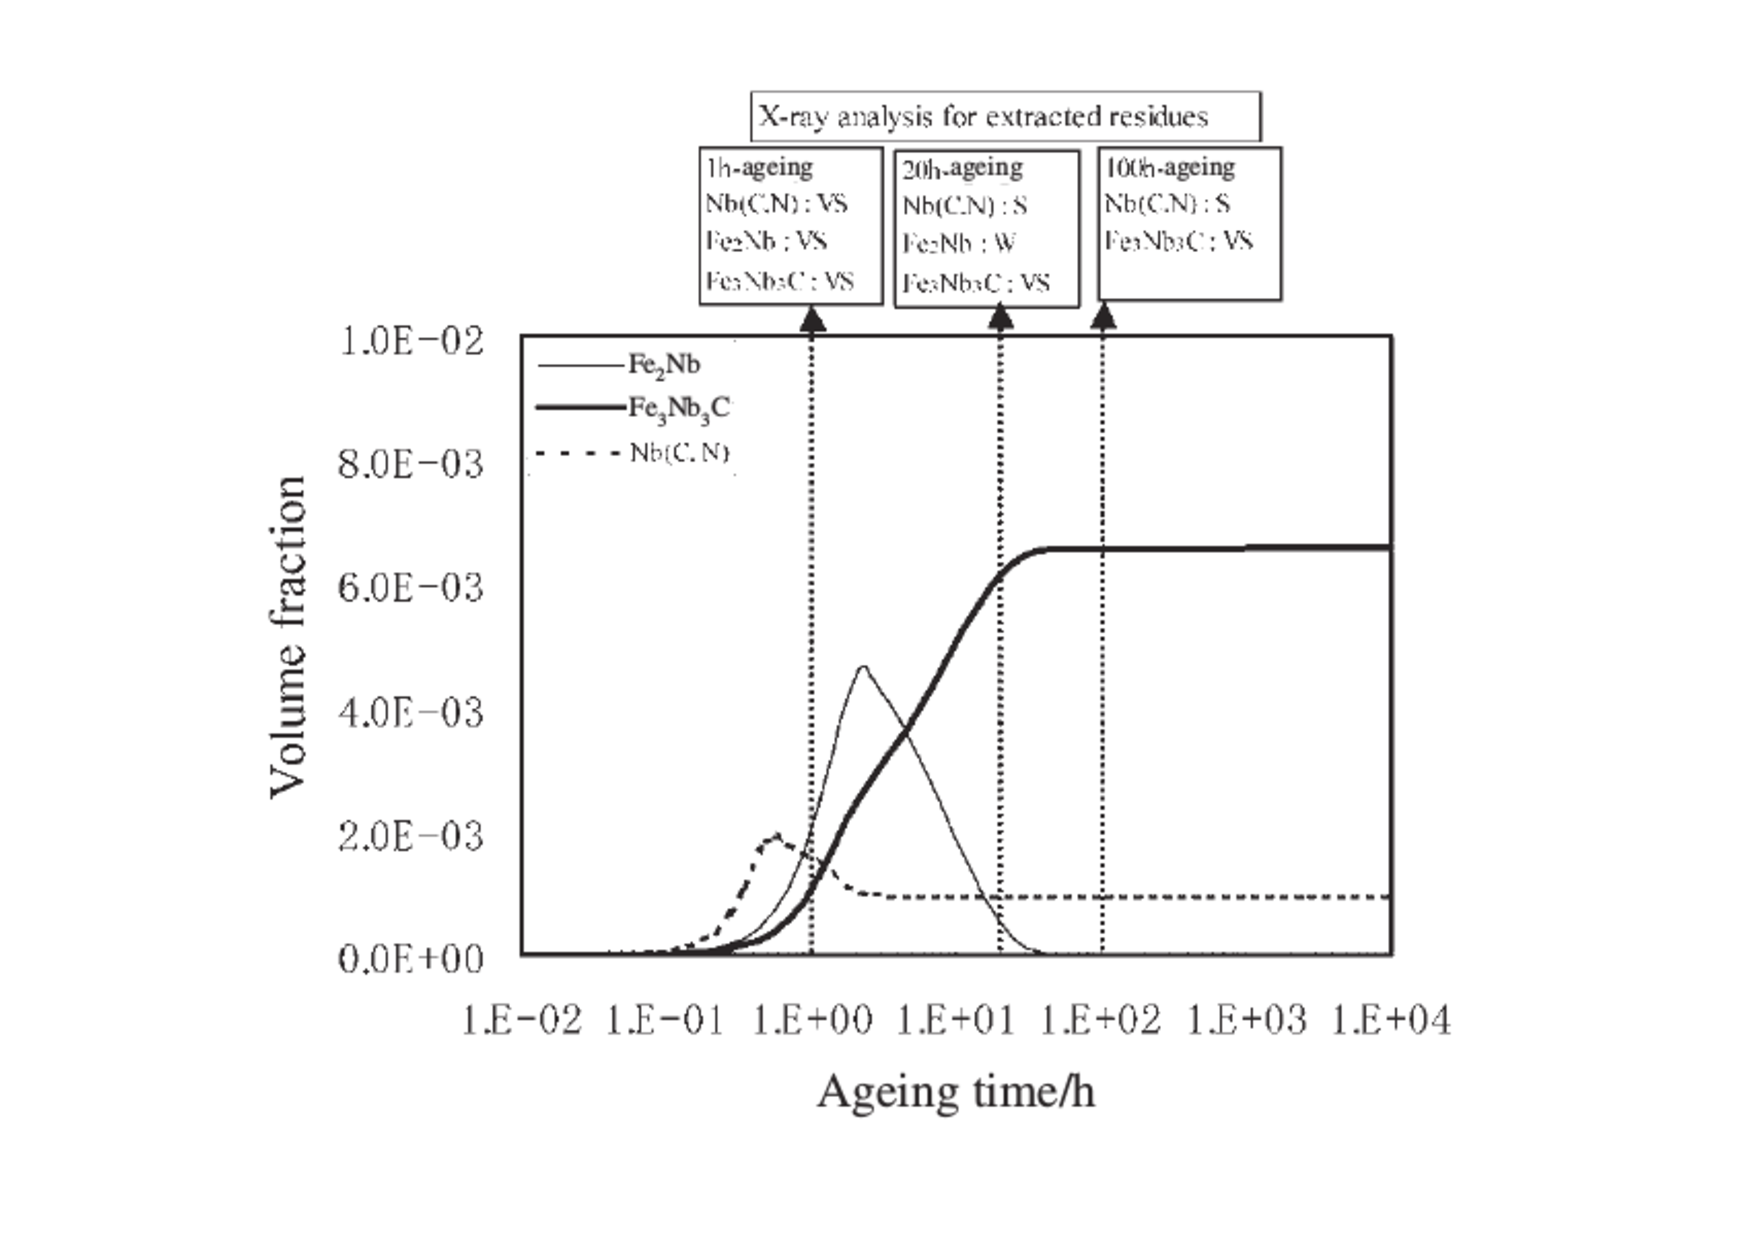
\includegraphics[width=14cm]{vol.pdf}
\caption{Volume fraction calculated as compared to experiments}
\label{fig:vol}
\end{figure}
%---------------------------------------
%--------------------------------------
\begin{figure}
\centering
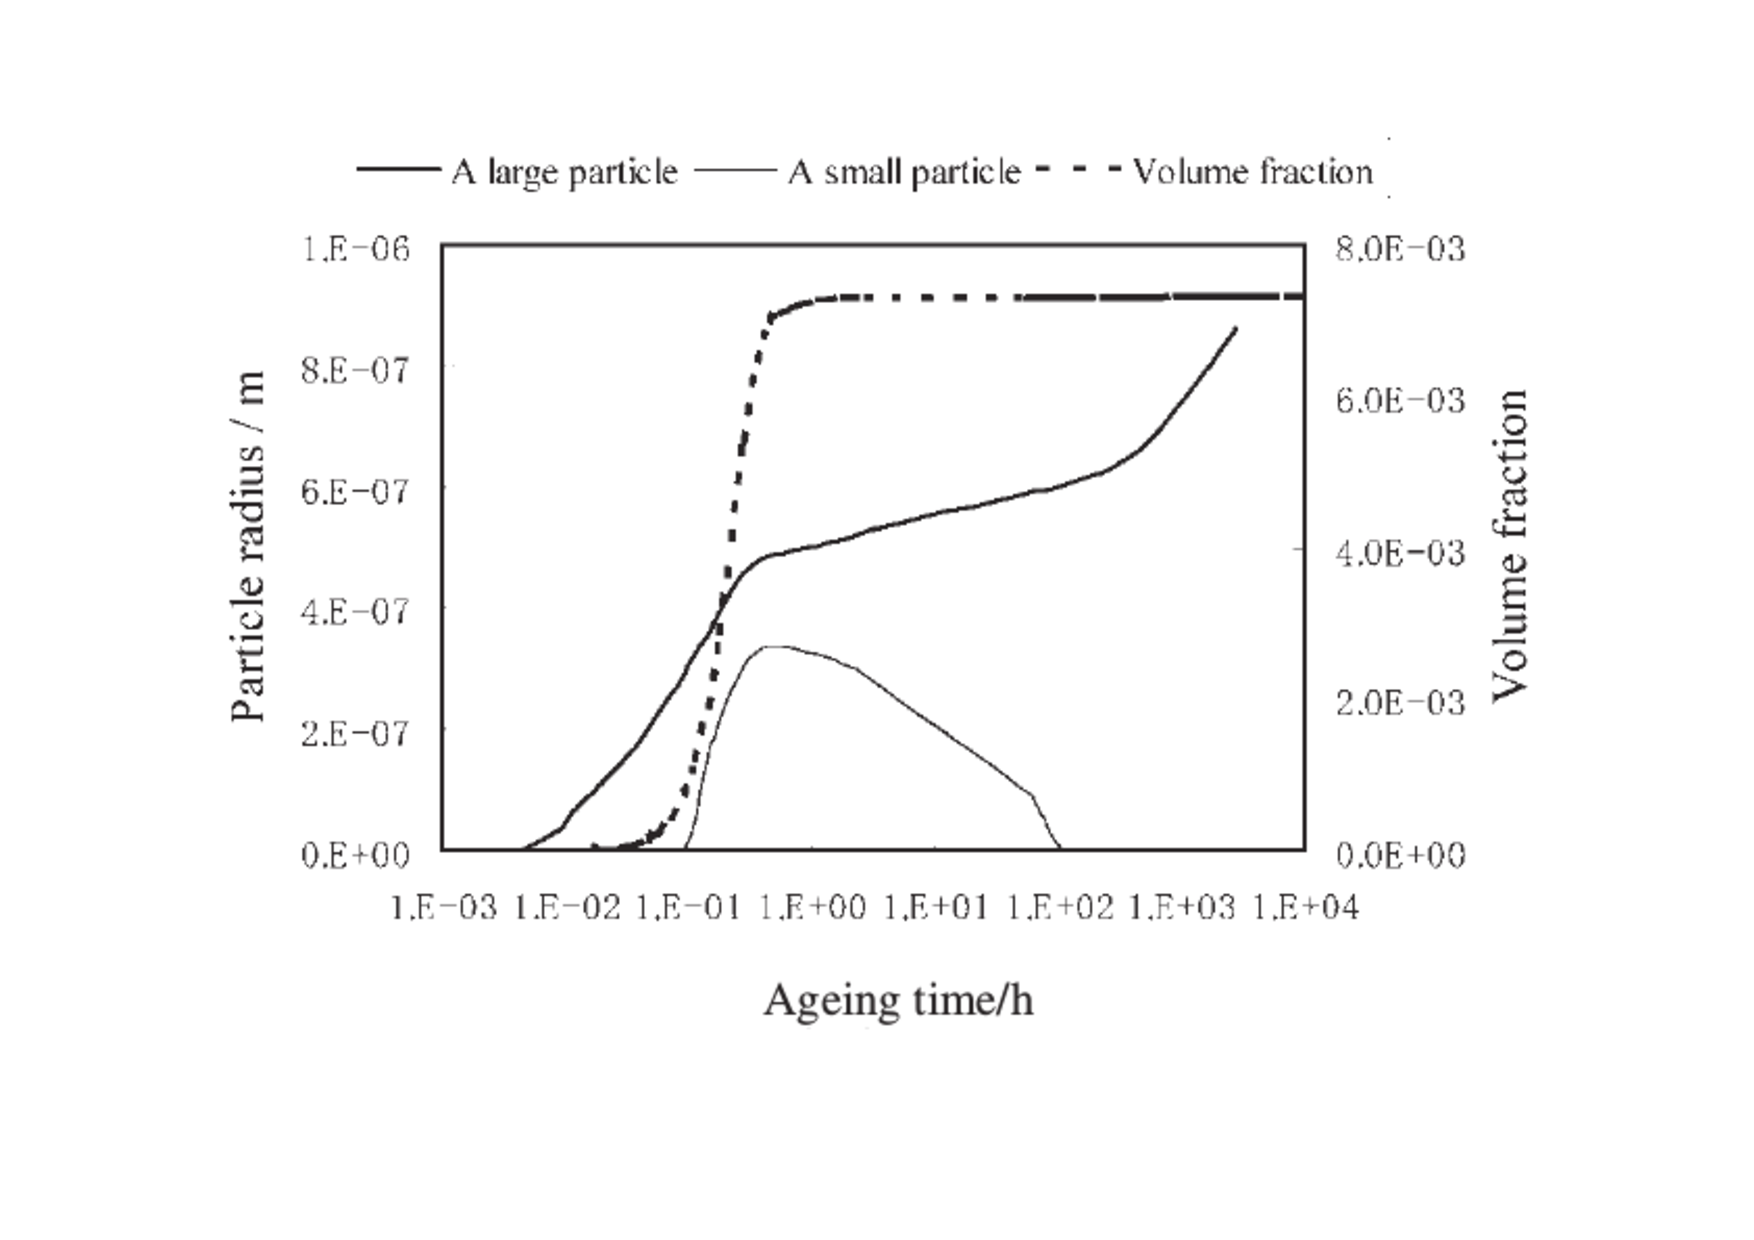
\includegraphics[width=14cm]{size.pdf}
\caption{Precipitate sizes calculated for Fe$_3$Nb$_3$C}
\label{fig:size}
\end{figure}
%---------------------------------------
\section{Conclusion}

It is observed that the most important parameter determining precipitation kinetics is that of the interfacial energy followed by the number of nucleating sites. Both the parameters were modeled using the classical theory to match with the experimental results. 




\end{document}
\grid
